\documentclass{article}
\usepackage{listings}
\usepackage{graphicx}
\usepackage{tabto}
\usepackage{amsmath}
\usepackage[backend=biber]{biblatex}
\usepackage{caption}
\usepackage{subcaption}
\usepackage[english]{babel}

% \addbibresource{oofdtd.bib}
% \bibliography{oofdtd}
\addbibresource{oofdtd.bib}
%\bibliographystyle{ieeetr}

\begin{document}


\title{Object-Oriented Finite-Difference Time-Domain}
\author{Dylan Pederson}

\maketitle

\section{Motivation}

\subsection{FDTD Algorithm}

Finite-Difference Time-Domain (FDTD) is a finite-difference method for solving Maxwell's equations directly in the time-domain. FDTD uses field values on a staggered grid 

	$$\nabla \times \vec{H} = \frac{\partial \vec{D}}{\partial t} + \vec{J}_e$$
	$$\nabla \times \vec{E} = -\frac{\partial \vec{B}}{\partial t} - \vec{J}_m$$ 
	$$\nabla \cdot \vec{D} = \rho_e $$ 
	$$\nabla \cdot \vec{B} = 0$$
	$$\vec{D} = \epsilon \vec{E} $$
    $$\vec{B} = \mu \vec{H} $$

The staggered grid has electric fields on the edges of a Yee cell, while the magnetic fields reside on the cell faces.

\begin{figure}[h]
\centering
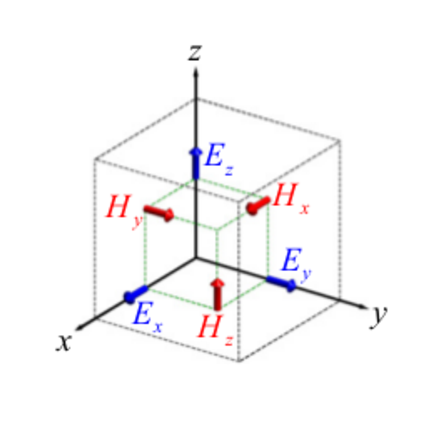
\includegraphics[scale=0.5]{figs/Yee_Grid3.eps}
\caption{Yee Cell and field placement}
\end{figure}

This is a natural arrangement for handling the curl terms in Maxwell's equations. We also use a leapfrog time-stepping scheme, where electric fields are updated at integer time steps, and magnetic fields are updated at half-integer time steps. This overall scheme is second order accurate in time and space (Note that just as in many explicit numerical schemes, there is a CFL criterion dictating a maximum time step size for a given spatial step size). For example, the update equation for $D_x$ is 

\begin{multline*} 
\frac{{D}_x|_{i+1/2,j,k}^{n+1} - {D}_x|_{i+1/2,j,k}^{n}}{\Delta t} = [\frac{{H}_z|_{i+1/2,j+1/2,k}^{n+1/2} - {H}_z|_{i+1/2,j-1/2,k}^{n+1/2}}{\Delta y} \\
- \frac{{H}_y|_{i+1/2,j,k+1/2}^{n+1/2} - {H}_y|_{i+1/2,j-1/2,k-1/2}^{n+1/2}}{\Delta z}] - c_0J_{e,x}|_{i+1/2,j,k}^{n+1/2}
\end{multline*} 




One of the main advantages of FDTD is that it preserves the divergence-free property of electric and magnetic fields in free space. In addition, boundary conditions are dealt with in a natural manner because of the edge/face placement of the fields. 

It turns out that there are many ways to incorporate advanced features into the FDTD framework. Some of these features include

\begin{itemize}
	\item radiation boundary condition
	\item arbirtrarily complex material dispersion
	\item plane wave source condition
	\item arbitrary source frequency content
\end{itemize}

Unfortunately, from a programming and code maintenance standpoint, the FDTD algorithm can quickly become unwieldy. A full object-oriented approach can make the programmer's job much easier. If each Yee cell is an object that knows how to update itself from its neighboring cells, then programming becomes easy. And by deriving classes from the base Yee cell class, a rich suite of features can be added at very little extra programming cost. For example, a material cell with Lorentzian dispersion may be added as a LorentzCell class that derives from the YeeCell class and changes the update functions. Then LorentzCell objects can be swapped into the grid with almost no hassle. However, the object-oriented approach is costly in terms of function call overhead and vtable lookups.  The approach using objects is known to run much slower than an approach more aligned with C programming. However, with parallelization, the object-oriented FDTD method can be competitive. And given enough processors, the runtime can become trivially short, even for very large problems. The aim of this project is to explore the possible speedup and runtimes for a parallelized object-oriented FDTD code. 


\subsection{Parallel Implementation}

In order to scale FDTD to very large grids, it must use domain decomposition. Then the logical approach to parallelization is to use data parallelism, and MPI. A simple way to decompose the full Yee grid is to separate the grid into cartesian processor blocks.

\begin{figure}[h]
\centering
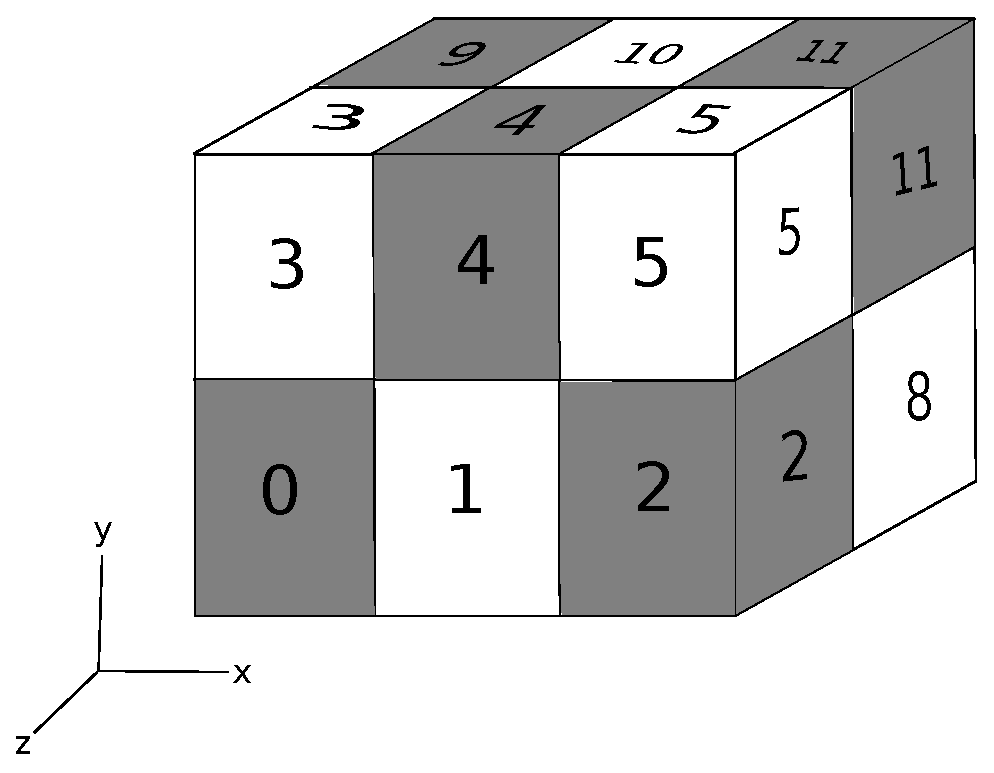
\includegraphics[scale=0.4]{figs/proc_grid.eps}
\caption{Example processor grid layout with 12 processes. The darker subdomains are colored black, and the white subdomains are colored red}
\end{figure}


The processors are colored either red or black, such that no two adjacent processors are of the same color. This will help prevent deadlock when communication happens. To facilitate easier communication and implementation of boundary conditions, each processor owns boundary cells that are located just outside of its physical domain.

\begin{figure}[h]
\centering
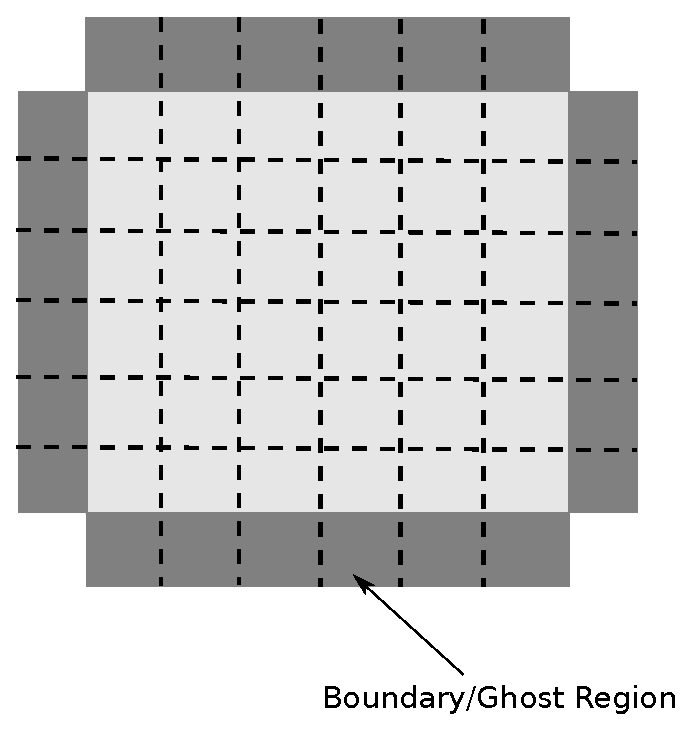
\includegraphics[scale=0.5]{figs/ghost_region.eps}
\caption{Definition of a ghost/boundary region in 2 dimensions}
\end{figure}


If these cells are on a processor-to-processor boundary, they are called \textit{Ghost Cells}. Ghost cells handle loading and grabbing data from a buffer that is sent between processes. If a processor subdomain is on the boundary of the overall domain, the boundary cells can be of one of many different types. If the domain is surrounded by a conductor, the boundary cells will be Perfect Electric Conductor (PEC) cells. If the domain has symmetry, the symmetry boundary will have Perfect Magnetic Conductor (PMC) cells. Other possibilities include Periodic boundaries and Bloch-Periodic boundaries. For the purpose of this study we will use only simple PEC boundaries, where the tangential E fields are zero. These are implemented by a PECCell object that overrides the update functions of a YeeCell.

To achieve parallelization without deadlock, on each time step every processor loops through its boundaries. If the processor is colored red, it communicates the given boundary. If the processor is colored black, it communicates the opposite of the given boundary. For example, if the current boundary is $X_{min}$, then red processors communicate $X_{min}$, while black processors communicate $X_{max}$. This ensures that pairwise communcation occurs during the communication steps. There are 6 communication steps per time step (one communication per field - $E_x$, $H_x$ etc...), and during each communication step, there are up to 6 seperate MPI SendRecv calls (one for each boundary). A snapshot of wave propagation calculated via FDTD is shown in the figure below. Note that the diagonal grid lines are artifacts of the software used for plotting.

\begin{figure}[h]
\centering
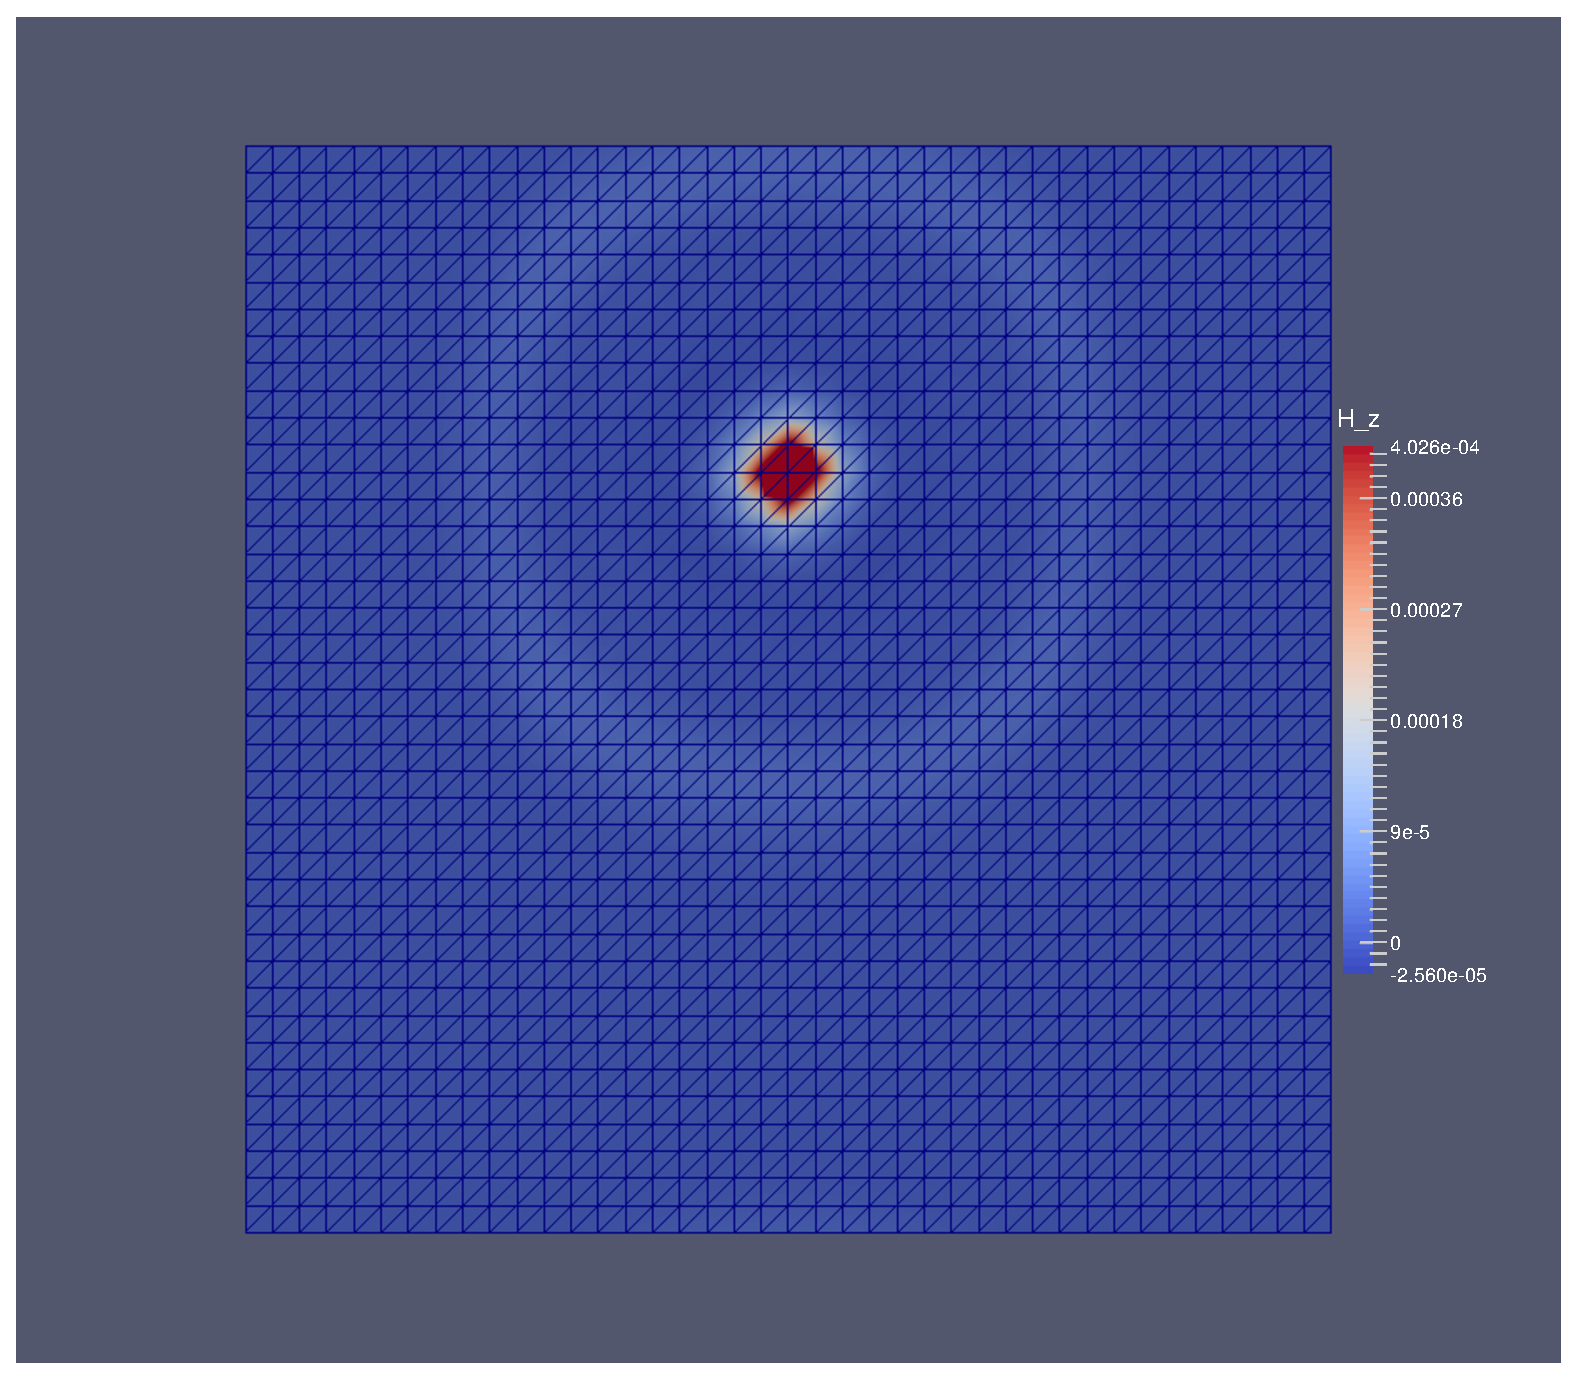
\includegraphics[scale=0.2]{figs/wave_propagation.eps}
\caption{Snapshot of wave propagation calculated by FDTD method. A sinusoidal source is placed in the domain just above the center}
\end{figure}


% \lstinputlisting[language=C++, firstline=30, lastline=44]{exchange_sort.cpp}

\section{Theoretical Issues}

We analyze the FDTD algorithm for a single time step by considering the standard metrics for parallel performance. First we define $N$ as the number of cells per dimension in the domain, and $P$ as the number of processors. The parallel FDTD algorithm does $N^3/P$ operations separately on each processor, then communicates $(N^3/P)^{2/3}$ cell values to each neighbor (assuming perfect cube subdomains). Knowing this, we can identify the following metrics for the FDTD parallel algorithm: \\
$$T_1 = N^3$$
$$T_P = \frac{N^3}{P} + 36(\alpha + \beta(\frac{N^3}{P})^{2/3})$$
$$S_P := \frac{T_1}{T_P} = \frac{1}{\frac{1}{P} + \frac{36\alpha}{N^3} + \frac{36\beta}{P^{2/3}N}}$$
$$E_P := \frac{S_P}{P} = \frac{1}{1 + \frac{36\alpha P}{N^3} + \frac{36\beta P^{1/3}}{N}}$$

Here, $\alpha$ and $\beta$ are the latency time and inverse bandwidth, respectively. Considering strong scaling ($N$=const., $P$ varies), the following is true as $P\rightarrow \infty$

$$S_P \rightarrow \frac{N^3}{36\alpha}$$
$$E_P \rightarrow \frac{N^3}{36\alpha P}$$

This is apparently does not scale well in the strong sense, because the parallel efficiency decreases with $P$. This is probably due to the increased communication cost for larger $P$. We also consider weak scaling, where the memory required per processor is held fixed (i.e. $\frac{N^3}{P}= const = M$), and see that the following relationships hold true.

$$S_P \rightarrow \frac{P}{1 + \frac{36\beta}{M^{1/3}} + \frac{36\alpha}{M}}$$
$$E_P \rightarrow \frac{1}{1 + \frac{36\beta}{M^{1/3}} + \frac{36\alpha}{M}}$$

These suggest that the parallel efficiency is a constant value for all $P$. Then the FDTD algorithm scales weakly according to this analysis. 

\section{Timing Results}

The performance of the OOFDTD code is evaluated through weak and strong scaling over 100 time steps in order to average out statistical fluctuations. In the strong scaling test, a free-space domain with 1,000,000 cells is excited by a sinusoidal source and allowed to propagate for 100 time steps. The domain is divided into $P=$(1,2,4,8,27,64,125,216,343,512, and 729) processors, with each processor assigned to one subdomain. In a weak scaling test, the same free-space domain and excitation is shared by $P$ processors with each processor receiving approximately 100,000 cells. Timing results were recorded and speedup/efficiency results are shown in Figs 5-7.

\begin{figure}[h]
\centering
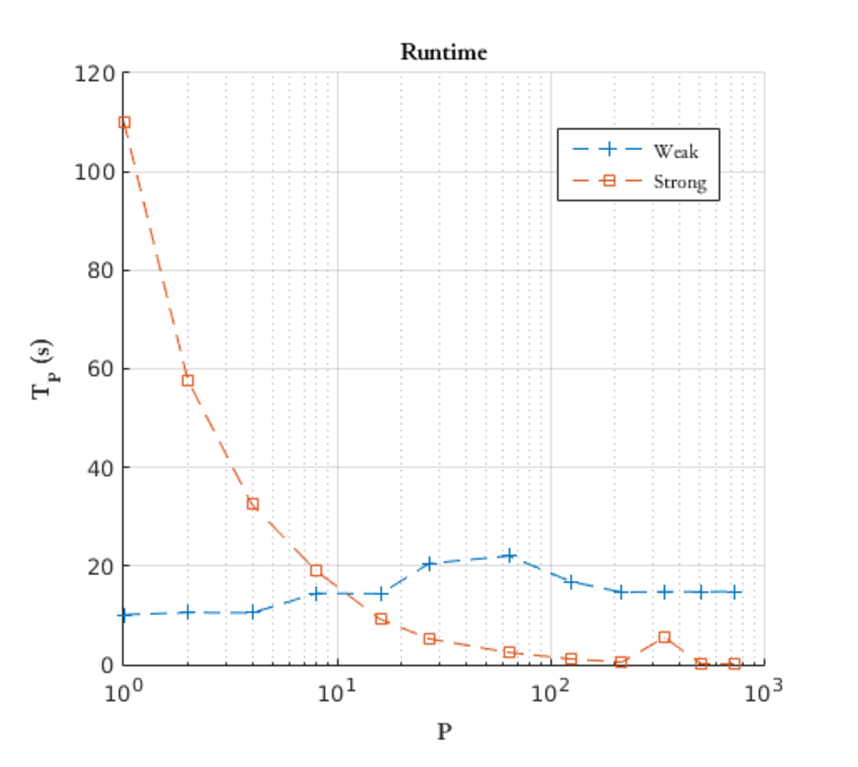
\includegraphics[scale=0.6]{figs/runtime.eps}
\caption{Total runtime scaling behavior for the FDTD algorithm.}
\end{figure}

\begin{figure}[!h]
\centering
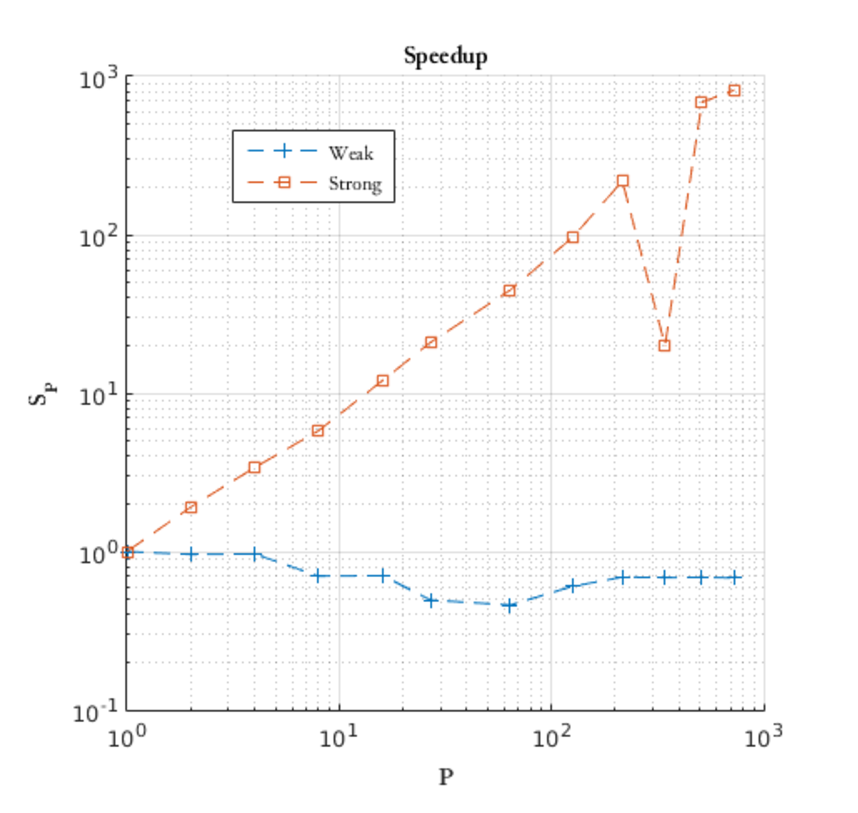
\includegraphics[scale=0.55]{figs/speedup.eps}
\caption{Speedup for the FDTD algorithm.}
\end{figure}

\begin{figure}[!h]
\centering
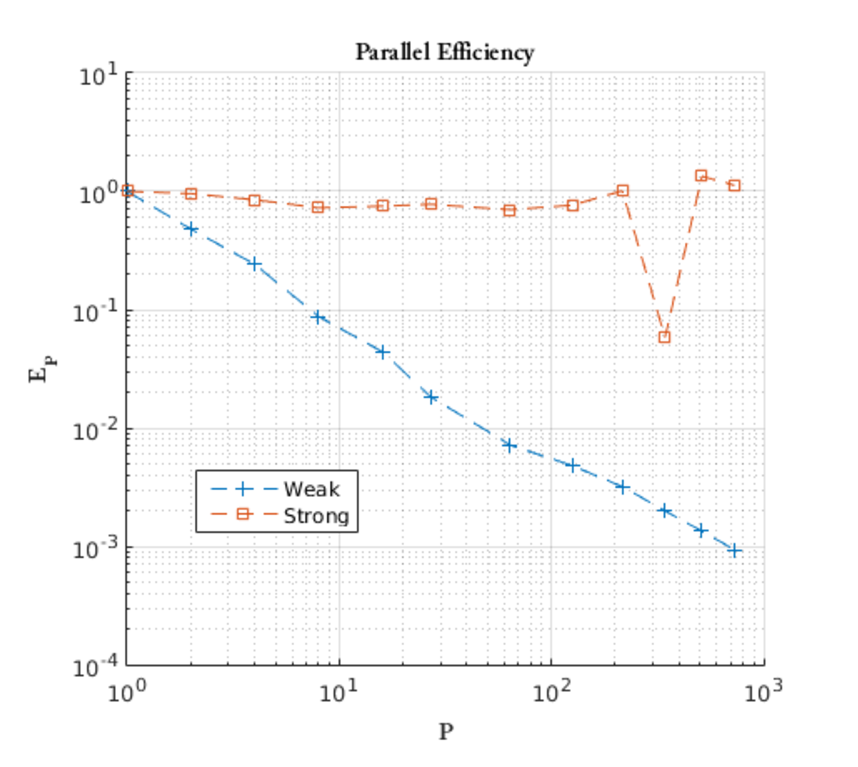
\includegraphics[scale=0.6]{figs/efficiency.eps}
\caption{Parallel Efficiency for the FDTD algorithm.}
\end{figure}

We immediately see that there is a problem...the results do not match the expected performance as outlined in the theory section! If we go back and look at the theory, we see that there are two problems with the analysis. First, the asymptotic analysis takes $P\rightarrow \infty$, where in reality, $P$ cannot be larger than $N^3$ (one cell per processor). And second, the weak scaling approximations use the end result from the strong scaling analysis. In reality, weak scaling will have a different form of $T_1$ and $T_P$, which will change that analysis completely. 

Let's revisit the strong scaling argument. If we recognize that

$$S_P^{strong} = \frac{P}{1 + \delta}$$
$$ \delta = 36 \alpha \frac{P}{N^3} + 36\beta(\frac{P}{N^3})^{1/3}$$

where $\delta$ is a small number (a decent approximation for the above numerical experiments), then by expanding the denominator and neglecting higher order terms

$$S_P^{strong} = P(1 - \delta)$$

and it follows that 

$$E_P^{strong} = 1-\delta$$

Now $S_P^{strong}$ and $E_P^{strong}$ have functional forms that match the results above. 

If we reformulate the weak scaling correctly, we identify

$$T_1 = M$$
$$T_P = M + 36(\alpha + \beta M^{2/3})$$
$$S_P^{weak} = \frac{M}{M + 36(\alpha + \beta M^{2/3})} = const. = K$$
$$E_P^{weak} = \frac{K}{P}$$

Again, this now matches the findings of the numerical experiments. So, the FDTD algorithm indeed scales strongly but not weakly. 

\section{Discussion}

The numerical experiments that were performed in this study show that the parallel OOFDTD algorithm scales strongly. This means that the performance penalty of using objects for flexibility can easily be overcome by using more processors for a given problem. As Fig. 5 shows, using 100 processors on a problem with 1,000,000 cells can solve the problem for 100 time steps in under 5 seconds. So, given a large number of processors, and a large problem size, the added programming convenience of using object-oriented design for FDTD software seems like a worthwhile venture. Of course, for smaller problems that don't require as many computational resources, it is best to stick with functional programming methods that avoid the overhead associated with objects. 

% \bibliography{oofdtd}
% \bibliographystyle{plain}
\nocite{*}
\printbibliography

\end{document}
